\documentclass[11pt,a4paper]{article}

\usepackage[margin=2.2cm]{geometry}
\usepackage[T1]{fontenc}
\usepackage{lmodern}
\usepackage{microtype}
\usepackage{booktabs,longtable,tabularx,array}
\usepackage{xcolor}
\usepackage{tikz}
\usetikzlibrary{arrows.meta,positioning,shapes.geometric,fit,backgrounds}
\usepackage{pifont}
\usepackage{enumitem}
\usepackage{caption}
\usepackage[hidelinks]{hyperref}
\usepackage{amsmath}

\definecolor{accent}{HTML}{1F4E79}
\definecolor{soft}{HTML}{DCE6F1}
\definecolor{bad}{HTML}{B00020}
\definecolor{good}{HTML}{2E7D32}
\newcommand{\cmark}{\textcolor{good}{\ding{51}}}
\newcommand{\xmark}{\textcolor{bad}{\ding{55}}}
\newcommand{\code}[1]{\texttt{\small #1}}
% \input is not expandable, so a rule right after it inside a tabular is "misplaced"; use the primitive
\makeatletter\newcommand{\inputrows}[1]{\@@input #1 }\makeatother
\setlist{itemsep=2pt,topsep=4pt}
\captionsetup{font=small,labelfont=bf}

\title{\textbf{A Multi-Agent Academic Helpdesk for IIT Jodhpur}\\[4pt]
\large Retrieval-augmented, tool-using agents on local 8B models --- design and evaluation}
\author{Sreenitya Thatikunta (B23CS1072)\\ CSL7650 Autonomous Systems, Semester I, AY 2026--27}
\date{October 2026}

\begin{document}
\maketitle

\begin{abstract}
We build an academic helpdesk that answers questions about IIT Jodhpur's programmes, course contents,
time table and academic rules, drafts emails to course instructors, cites the document behind every
answer, and refuses --- and logs for a human --- anything it cannot answer. The system runs entirely on a
16\,GB laptop: Google ADK agents call Ollama-hosted 8B models (Qwen3, Llama~3.1) through LiteLLM, with
hybrid retrieval (dense \code{nomic-embed-text} + BM25) over ChromaDB and structured tools over the
semester's course and exam data. The knowledge base contains 33 real documents (1{,}134 chunks). We compare
a single-agent baseline with a multi-agent version (router + policy, schedule and email specialists) on 30
prompts (31 turns) $\times$ 2 models $\times$ 2 modes $\times$ 3 repeats. Qwen3 reaches 87\% accuracy (single)
and 78\% groundedness (multi), Llama~3.1 65--69\%; out-of-scope refusals are 100\% correct and logged in
all configurations. Model choice matters more than architecture; the multi-agent design improves grounding
but introduces router- and specialist-specific failure modes. We also report an ADK behaviour that silently
overrides specialist instructions in small models, and the data-level techniques (an amendment register for
superseded rules, scoped search, deterministic guards) that mattered more than prompt wording.
\end{abstract}

\tableofcontents
\bigskip

%=====================================================================
\section{Problem}
%=====================================================================
The assignment asks for a multi-agent \emph{Academic Helpdesk Agent} that
(i) answers questions about academic programmes, course contents, and rules and regulations, e.g.
\emph{``What is the attendance requirement to sit in the Major exam?''}, \emph{``What is the slot for the course
Autonomous Systems?''}, \emph{``How many 400-level electives have been floated by the Humanities department this
semester?''}, \emph{``How many Open Elective credits do I need for a B.Tech?''};
(ii) drafts an email to a course instructor (sick leave, make-up permission), e.g.
\emph{``Write an email to the course instructor of CSL7570 that I need leave for 2 days''};
(iii) answers \emph{``I don't know''} to anything else (\emph{``What are the dining options on campus?''}) and
logs such questions for a human; and (iv) cites the source document of every answer.
It must use RAG with a local embedding model and vector store, tools (vector search, time-table and course
lookup from CSV, instructor email lookup, email drafting), Google ADK with Ollama-hosted 8B models, run on
16\,GB of RAM, start as a single agent and then become an orchestrator with policy, schedule and email
agents, and be evaluated on 20--30 prompts for accuracy, groundedness and correct refusals, across models and
repeated runs.

%=====================================================================
\section{Data}
%=====================================================================
\subsection{Documents}
We collected 33 real documents (Table~\ref{tab:data}). 24 are public pages and PDFs from
\code{iitj.ac.in}; 9 come from the author's institute mailbox (Registration and Examination Cell
circulars) because the current time table, course list and IH lists are not public. Three scanned
circulars were OCR'd with Tesseract. Every document is described in \code{data/manifest.csv} with a
title, category, source, date and a \emph{status}: 29 are \emph{current}, 4 \emph{superseded} by newer
versions (2018 B.Tech regulations, 2025--26 calendar, 2023 slot chart, the previous year's IH list).

\begin{table}[h]
\centering\small
\begin{tabularx}{\linewidth}{l c X}
\toprule
Category & \# & Examples \\
\midrule
Regulations & 5 & Academic Regulations 2019 (PDF + web), B.Tech Regulations 2018, PG Regulations 2022+, MS by Research \\
Circulars / orders & 5 & Circular 51 (attendance, 2024), Circular 52 (exam policy, 2024), M.Tech norms, announcements \\
Curricula & 5 & B.Tech CSE (pre-2026 batches), AIDE 2026+, EE 2025+, M.Tech AI, M.Tech CSE \\
Course catalogues & 8 & CSE course details, HSS concept note, common courses, IH2/IH3 syllabi, IH course lists \\
Calendars & 3 & AY 2026--27, AY 2025--26, Summer 2026 \\
Time tables & 3 & Finalized course list, slot system + classroom allocation + minor-exam grid, 2023 slot chart \\
Exams & 2 & Major-exam time table Sem I 2026--27, New Guidelines for Institute Examination (2024) \\
Registration & 2 & UG registration guidelines, Circular 2283 \\
\bottomrule
\end{tabularx}
\caption{The 33 source documents by category.}
\label{tab:data}
\end{table}

\subsection{Structured data}
The semester spreadsheets are converted to CSVs: \code{courses.csv} (821 offerings from the final
classroom allocation plus the finalized course list, with slot, classroom, instructor, level and an
\code{ih\_group} tag so that ``Humanities'' means \emph{Institute Humanities}, including IH courses taught by
AIDE), \code{slots.csv} (slot $\rightarrow$ day and time), \code{exam\_schedule.csv} (45 minor + 44 major exam
slot entries) and \code{faculty.csv} (312 instructors). \textbf{All email addresses are dummy values}
(\code{first.last@iitj.example}, a reserved domain); other addresses in the documents are masked at ingestion,
and sheets listing other students were not collected.

\subsection{Amendment register}
Institutional rules are amended by later circulars while the old text stays in the regulations.
\code{data/amendments.csv} lists passages superseded by a named newer document (e.g.\ the 2019 attendance rule
$\rightarrow$ Circular~51; the 2019/2022 make-up rules $\rightarrow$ the 2024 Examination Guidelines); matching chunks are
marked \emph{amended} and never retrieved.

%=====================================================================
\section{System design}
%=====================================================================
\subsection{Retrieval pipeline}
Documents are loaded page by page (PDF, OCR text, HTML with tables rendered as rows, spreadsheets per
sheet), chunked to $\sim$1{,}800 characters with 250 overlap (documents under 3{,}200 characters stay whole so a
circular's ``existing'' and ``revised'' policy are not separated), prefixed with a contextual header
\code{[title | date | page]}, embedded with \code{nomic-embed-text} and stored in ChromaDB.
A query runs dense (top 30) and BM25 (top 30) retrieval, fused with reciprocal rank fusion; amended chunks
are dropped, superseded documents get half weight, at most two chunks per document are returned, and if the
best dense distance exceeds 0.35 the search reports \emph{not found}. A \code{document} filter restricts the
search to one document (e.g.\ a programme's curriculum).

\begin{figure}[h]
\centering
\resizebox{\linewidth}{!}{%
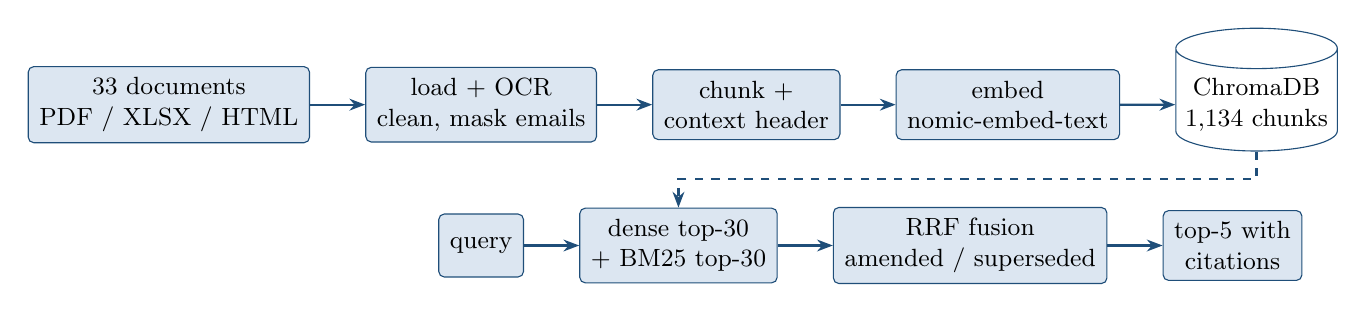
\begin{tikzpicture}[node distance=5mm and 7mm, font=\small,
  box/.style={draw=accent, fill=soft, rounded corners=2pt, minimum height=8mm, align=center, inner sep=4pt},
  db/.style={draw=accent, fill=white, cylinder, shape border rotate=90, aspect=0.25, minimum height=11mm, align=center},
  arr/.style={-{Stealth[length=2mm]}, thick, accent}]
\node[box] (raw) {33 documents\\PDF / XLSX / HTML};
\node[box, right=of raw] (load) {load + OCR\\clean, mask emails};
\node[box, right=of load] (chunk) {chunk +\\context header};
\node[box, right=of chunk] (emb) {embed\\nomic-embed-text};
\node[db, right=of emb] (chroma) {ChromaDB\\1{,}134 chunks};
\node[box, below=9mm of load] (q) {query};
\node[box, right=of q] (dense) {dense top-30\\+ BM25 top-30};
\node[box, right=of dense] (rrf) {RRF fusion\\amended / superseded};
\node[box, right=of rrf] (out) {top-5 with\\citations};
\draw[arr] (raw)--(load); \draw[arr] (load)--(chunk); \draw[arr] (chunk)--(emb); \draw[arr] (emb)--(chroma);
\draw[arr] (q)--(dense); \draw[arr] (dense)--(rrf); \draw[arr] (rrf)--(out);
\draw[arr, dashed] (chroma.south) -- ++(0,-0.35) -| (dense.north);
\end{tikzpicture}}
\caption{Ingestion (top) and hybrid retrieval (bottom); retrieval reads the ChromaDB index (dashed).}
\end{figure}

Retrieval was tuned on a separate 19-question check: dense-only search placed the right document first
for 9/18 questions (17/18 in the top 5); BM25 alone made it worse (15/18) until contextual headers gave
keywords something to match; the final pipeline reaches 12/19 at rank 1 and 18/19 in the top 5. Best-match
distances of in-scope (0.15--0.28) and out-of-scope questions (0.26--0.43) overlap, so the distance threshold
rejects only half of the out-of-scope questions --- refusals must come from the agents.

\subsection{Tools}
\noindent\begin{minipage}{\linewidth}
\centering\small
\begin{tabularx}{\linewidth}{l X}
\toprule
Tool & Behaviour \\
\midrule
\code{search\_documents} & hybrid RAG search; passages with citation, date, status \\
\code{lookup\_course} & course by code or name; unknown codes return ``did you mean'' suggestions (CSL7570 $\rightarrow$ CSL7650) \\
\code{get\_slot} & slot, weekly class times, classroom, instructors, minor/major exam date \\
\code{list\_courses} & count and list of courses floated by department / level (``Humanities'' = IH) \\
\code{get\_instructor\_email} & instructor and (dummy) email by course or name \\
\code{draft\_email} & saves the draft to \code{drafts/} with a NOT SENT header; never sends \\
\code{log\_unanswered\_question} & appends the question to \code{logs/unanswered.jsonl} for a human \\
\bottomrule
\end{tabularx}
\captionof{table}{Agent tools (plain Python functions; ADK derives the schemas from type hints and docstrings).}
\end{minipage}
\medskip

\subsection{Agents}
The \textbf{single agent} is one ADK \code{LlmAgent} with all seven tools and a prompt composed of blocks:
scope, \emph{call a tool before every answer}, grounding rules (exact refusal sentence + log; a related
passage is not an answer; the newest source and the revised policy win; cite 1--2 sources), and sections for
policy, schedule and email questions. The \textbf{multi-agent} version (Figure~\ref{fig:agents}) has a router
that calls \code{transfer\_to\_agent} or refuses, and three specialists that see only their own tools and
rules. Models run with temperature 0.2 and an 8{,}192-token context; Qwen3 runs with thinking disabled
(\code{think=False}), which removed leaked reasoning from its answers and cut latency tenfold.

\begin{figure}[h]
\centering
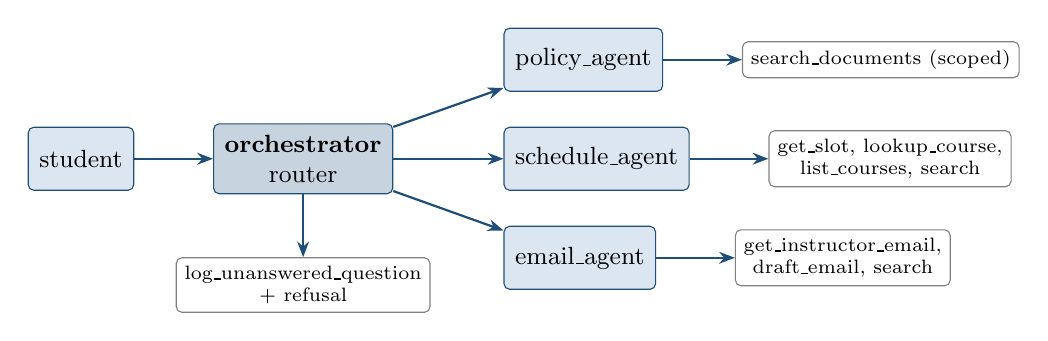
\begin{tikzpicture}[node distance=6mm and 10mm, font=\small,
  box/.style={draw=accent, fill=soft, rounded corners=2pt, minimum height=8mm, align=center, inner sep=4pt},
  tool/.style={draw=gray, fill=white, rounded corners=2pt, align=center, font=\scriptsize, inner sep=3pt},
  arr/.style={-{Stealth[length=2mm]}, thick, accent}]
\node[box] (s) {student};
\node[box, right=of s, fill=accent!25] (o) {\textbf{orchestrator}\\router};
\node[box, above right=4mm and 14mm of o] (p) {policy\_agent};
\node[box, right=14mm of o] (sc) {schedule\_agent};
\node[box, below right=4mm and 14mm of o] (e) {email\_agent};
\node[tool, right=of p] (pt) {search\_documents (scoped)};
\node[tool, right=of sc] (st) {get\_slot, lookup\_course,\\list\_courses, search};
\node[tool, right=of e] (et) {get\_instructor\_email,\\draft\_email, search};
\node[tool, below=8mm of o] (log) {log\_unanswered\_question\\+ refusal};
\draw[arr] (s)--(o); \draw[arr] (o)--(p); \draw[arr] (o)--(sc); \draw[arr] (o)--(e);
\draw[arr] (p)--(pt); \draw[arr] (sc)--(st); \draw[arr] (e)--(et); \draw[arr] (o)--(log);
\end{tikzpicture}
\caption{Multi-agent design. Only the router transfers; every new student message returns to it.}
\label{fig:agents}
\end{figure}

\subsection{Guards}
Two deterministic callbacks wrap every agent. (1) If a model writes the refusal sentence without calling
\code{log\_unanswered\_question} --- Qwen3 did so in about half of its refusals during development --- the
question is logged in code, so every unanswered question reaches a human. (2) Tool calls that Llama~3.1 prints as
JSON text are stripped from the answer.

%=====================================================================
\section{Engineering findings during development}
%=====================================================================
\paragraph{Prompt rules are not enough for 8B models.} The first single-agent run answered the attendance
and Open Elective questions \emph{without calling any tool}, with invented citations. A \emph{tools-first}
block fixed tool use, but grounded answers were still wrong when old and new versions of a rule were both
retrieved: three of five passages for the attendance question stated the 2019 rule. The amendment register,
keeping short circulars whole and the per-document cap fixed this where prompt wording (``the newest source
wins'') had not.

\paragraph{Parameters a small model can misuse should be removed.} A \code{course\_type} filter turned
``3 Humanities electives'' into 0 (most departments leave the category blank), and the \code{document}
filter was used unprompted to scope rule questions to the wrong document. Both were removed from the agents
that misused them.

\paragraph{ADK's transfer instructions override specialist rules.} In multi-agent mode the policy agent never
asked for the student's programme (0/3), although its prompt alone did (3/3). The LLM request showed that,
when an agent is allowed to transfer, ADK appends generic instructions to the \emph{end} of its system prompt
(\emph{``If you are the best to answer the question according to your description, you can answer it''}) and adds
a \code{transfer\_to\_agent} tool. Removing the transfer bookkeeping messages did not help; disabling transfers
from specialists did (3/3, then 5/5). Only the router routes, and multi-turn conversations still work because
each new message is routed again.

\paragraph{Programme- and batch-dependent answers need clarification.} Open Elective credits are 10 in the
2019 regulations and the CSE curriculum but 12 in the newer EE and AIDE curricula. The agent therefore asks
for the branch and year of joining and then searches only that curriculum (``B.Tech CSE, joined 2023''
$\rightarrow$ 10 credits).

%=====================================================================
\section{Evaluation methodology}
%=====================================================================
The evaluation set has 30 items (31 turns, Appendix~\ref{app:questions}): policy 9, schedule 5, course counts 3,
email 4, out-of-scope 6, multi-intent 2, and one two-turn conversation; it contains all five assignment examples.
Every expected answer was checked against the documents or tools. Each turn specifies an expected
\emph{behaviour} (answer, refuse, draft, suggest, clarify), regular expressions for the required facts,
forbidden patterns for superseded rules, acceptable citation sources, the relevant tools, and the expected
specialist. Each of the 12 configurations (2 models $\times$ 2 modes $\times$ 3 repeats) ran all items in fresh
sessions with its own draft folder and unanswered log (372 turns, no errors).

\begin{itemize}
\item \textbf{Accuracy}: the expected behaviour is met (facts present and no superseded rule; refusal; a
clarifying question without a credit number; a suggestion without drafting; a saved draft to the right recipient).
\item \textbf{Groundedness} (answer and draft turns): correct, the relevant tool was called, and an expected
source is cited (for drafts: the recipient came from the instructor lookup).
\item \textbf{Refusals}: correct-refusal rate on out-of-scope items, false-refusal rate on the rest, logging rate.
\item \textbf{Routing}: the first specialist the router transfers to is the expected one.
\item \textbf{Consistency}: whether correctness, or the facts the question asks for, differ across repeats.
\end{itemize}

Every turn scored wrong or ungrounded was read by hand. This found three errors in the answer key, corrected for all
configurations: the PhD maximum duration \emph{is} stated in the PG Regulations (\S11.5, 14 registered semesters;
the item had been designed as unanswerable after a keyword search for ``years'' missed it), and two
over-literal patterns (``two exams: Minor and Major''; a quoted ``I''~grade). No per-answer overrides were needed.

%=====================================================================
\section{Results}
%=====================================================================
\begin{table}[h]
\centering\small
\resizebox{\linewidth}{!}{%
\begin{tabular}{l c c c c c c}
\toprule
Config & Accuracy & Grounded & Correct ref. & False ref. & Routing & Latency mean / p90 (s) \\
\midrule
\inputrows{tables/headline.tex}
\bottomrule
\end{tabular}}
\caption{Headline metrics, all repeats pooled (93 turns per configuration; 69 answer/draft turns for
groundedness; 18 out-of-scope turns). All refused out-of-scope questions were logged.}
\label{tab:headline}
\end{table}

\begin{figure}[h]
\centering
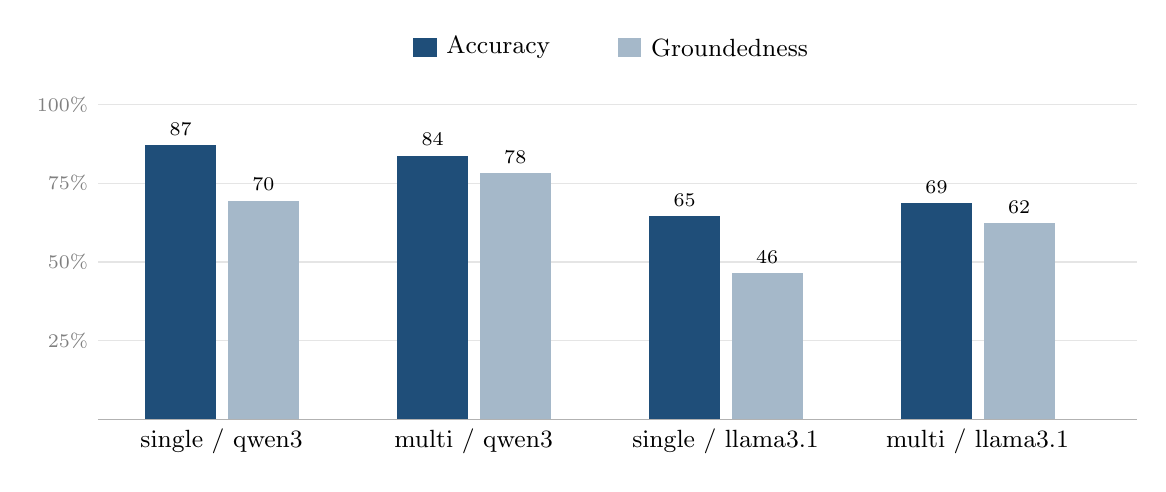
\begin{tikzpicture}[font=\small]
\draw[gray!60] (0,0) -- (13.2,0);
\draw[gray!20] (0,1.00) -- (13.2,1.00); \node[left,font=\scriptsize,gray] at (0,1.00) {25\%};
\draw[gray!20] (0,2.00) -- (13.2,2.00); \node[left,font=\scriptsize,gray] at (0,2.00) {50\%};
\draw[gray!20] (0,3.00) -- (13.2,3.00); \node[left,font=\scriptsize,gray] at (0,3.00) {75\%};
\draw[gray!20] (0,4.00) -- (13.2,4.00); \node[left,font=\scriptsize,gray] at (0,4.00) {100\%};
\fill[accent] (0.60,0) rectangle (1.50,3.48); \node[above,font=\scriptsize] at (1.05,3.48) {87};
\fill[accent!40] (1.65,0) rectangle (2.55,2.78); \node[above,font=\scriptsize] at (2.10,2.78) {70};
\node[below] at (1.57,0) {single / qwen3};
\fill[accent] (3.80,0) rectangle (4.70,3.35); \node[above,font=\scriptsize] at (4.25,3.35) {84};
\fill[accent!40] (4.85,0) rectangle (5.75,3.13); \node[above,font=\scriptsize] at (5.30,3.13) {78};
\node[below] at (4.77,0) {multi / qwen3};
\fill[accent] (7.00,0) rectangle (7.90,2.58); \node[above,font=\scriptsize] at (7.45,2.58) {65};
\fill[accent!40] (8.05,0) rectangle (8.95,1.86); \node[above,font=\scriptsize] at (8.50,1.86) {46};
\node[below] at (7.97,0) {single / llama3.1};
\fill[accent] (10.20,0) rectangle (11.10,2.75); \node[above,font=\scriptsize] at (10.65,2.75) {69};
\fill[accent!40] (11.25,0) rectangle (12.15,2.49); \node[above,font=\scriptsize] at (11.70,2.49) {62};
\node[below] at (11.17,0) {multi / llama3.1};
\fill[accent] (4.0,4.6) rectangle (4.3,4.85); \node[right] at (4.3,4.72) {Accuracy};
\fill[accent!40] (6.6,4.6) rectangle (6.9,4.85); \node[right] at (6.9,4.72) {Groundedness};
\end{tikzpicture}

\caption{Accuracy and groundedness per configuration.}
\end{figure}

\begin{table}[h]
\centering\small
\begin{tabular}{l c c c c c c c}
\toprule
Config & Policy & Schedule & Count & Email & Out of scope & Multi-intent & Conversation \\
\midrule
\inputrows{tables/category.tex}
\bottomrule
\end{tabular}
\caption{Accuracy (\%) by category.}
\end{table}

\begin{table}[h]
\centering\small
\begin{tabular}{l c c}
\toprule
Config & Unstable correctness & Answer changed \\
\midrule
\inputrows{tables/consistency.tex}
\bottomrule
\end{tabular}
\caption{Consistency across the three repeats (31 turns). \emph{Answer changed}: the facts the question asks for
differ between repeats.}
\end{table}

\subsection*{Questions whose answers changed across runs}
\begin{longtable}{l l c p{7.2cm}}
\toprule
Config & Item & Correct (r1 r2 r3) & Asked-for facts per repeat \\
\midrule
\endhead
\inputrows{tables/changed.tex}
\bottomrule
\end{longtable}
Qwen3 gave the same asked-for facts in every repeat in both modes; all changes are Llama~3.1's
(e.g.\ V01: asking for the programme in two repeats but not the third; P09: ``14 semesters'' twice and an
invented ``4--5 years'' once).

\subsection*{Routing errors (multi-agent)}
\noindent\begin{minipage}{\linewidth}
\centering\small
\begin{tabular}{l l l c}
\toprule
Config & Item & Routed to & Repeats \\
\midrule
\inputrows{tables/misroutes.tex}
\bottomrule
\end{tabular}
\captionof{table}{All routing errors are systematic (the same item in every repeat). For Qwen3 P09 and S02 the router
handled the request itself --- a refusal and an empty reply respectively.}
\end{minipage}

%=====================================================================
\section{Analysis}
%=====================================================================
\paragraph{Model choice matters more than architecture.} Qwen3 (thinking disabled) beats Llama~3.1 by
15--22 accuracy points in both modes, is faster in single mode, and is fully stable across repeats.
Llama~3.1 never called \code{draft\_email} in any of its 24 draft requests --- it asked again for details the
student had already given or wrote the email into the chat --- and answered the attendance question with the
\emph{existing} policy quoted inside Circular~51 in all six runs.

\paragraph{Multi-agent improves grounding, not necessarily accuracy.} Focused specialists search and cite more
consistently (groundedness +8 points for Qwen3, +16 for Llama~3.1), and for Llama~3.1 accuracy (+4) and
stability (answers changed on 3 instead of 8 questions) also improve. For Qwen3 accuracy drops by 3 points
through three failure modes that do not exist in the single agent: the router returning an empty reply (S02),
a specialist refusing a syllabus question whose answer it had retrieved (P08), and the router refusing an
in-scope question itself (P09). The extra routing step adds about 2.7\,s on average for Qwen3.

\paragraph{Refusals.} Out-of-scope questions are refused and logged in every configuration (72/72); the
deterministic guard makes the logging independent of the model. The remaining problem is \emph{false}
refusals of answerable questions (8\% for multi-agent Qwen3).

\paragraph{Groundedness vs.\ accuracy.} Several answers were right but ungrounded: Qwen3 answered the I-grade
question without any tool call and cited a non-existent ``Academic Regulations 2026--27, Section~4.3''; the
attendance half of a mixed request was answered from the model's own knowledge. Reporting groundedness separately
exposes answers that are right by luck.

\paragraph{Hardest items.} The IH2 course count failed everywhere (0/12): models read ``5th semester'' as
500-level courses, and \code{list\_courses} cannot filter by IH group. The make-up rule + email request failed
everywhere (0/12): the single agent skipped the draft, and the multi-agent Qwen3 drafted correctly but omitted the
10-day deadline.

%=====================================================================
\section{Limitations and future work}
%=====================================================================
\begin{itemize}
\item Add IH-group and semester filters to \code{list\_courses}; add a router fallback when the router returns no
text and no transfer; soften the ``related passage is not an answer'' rule for syllabus questions.
\item The distance threshold separates out-of-scope queries poorly; an LLM relevance check on the top passage or a
small classifier could replace it.
\item Regex scoring needed three answer-key corrections; an LLM judge with human spot checks would scale better.
\item Time tables are tentative and semester-specific; the (idempotent) data pipeline must be re-run each semester.
\item Only two 8B models were compared; larger or tool-tuned models are the obvious next step.
\end{itemize}

%=====================================================================
\section{Conclusion}
%=====================================================================
A fully local helpdesk on 8B models can answer most academic questions correctly with citations, refuse and log
everything outside its scope, and draft instructor emails safely. With Qwen3 it reaches 87\% accuracy (single
agent) and 78\% groundedness (multi-agent) with stable answers across runs. The improvements that mattered most
were in the data and tools --- explicit recency through an amendment register, scoped search, removing
misusable parameters, deterministic guards --- and in understanding what the agent framework adds to the prompt.
The multi-agent architecture improves grounding but needs its own safeguards against router and specialist failures.

\bigskip
\noindent\textbf{Code and data:} the repository README describes setup and reproduction; \code{docs/TECHNICAL.md}
gives the technical details and \code{docs/PROGRESS\_LOG.md} the full development log.

\appendix
%=====================================================================
\section{Evaluation questions}\label{app:questions}
%=====================================================================
{\small
\begin{longtable}{l l p{5.6cm} p{6.3cm}}
\toprule
Item & Category & Question & Expected \\
\midrule
\endhead
\inputrows{tables/questions.tex}
\bottomrule
\end{longtable}}

%=====================================================================
\section{Per-question results}
%=====================================================================
Correct runs out of 3 repeats (\textbf{bold}: all correct; \textcolor{bad}{red}: none correct).

{\small
\begin{longtable}{l c c c c}
\toprule
Item & single / qwen3 & multi / qwen3 & single / llama3.1 & multi / llama3.1 \\
\midrule
\endhead
\inputrows{tables/perquestion.tex}
\bottomrule
\end{longtable}}

\end{document}
